%% BioMed_Central_Tex_Template_v1.06
%%                                      %
%  bmc_article.tex            ver: 1.06 %
%                                       %

%%IMPORTANT: do not delete the first line of this template
%%It must be present to enable the BMC Submission system to 
%%recognise this template!!

%%%%%%%%%%%%%%%%%%%%%%%%%%%%%%%%%%%%%%%%%
%%                                     %%
%%  LaTeX template for BioMed Central  %%
%%     journal article submissions     %%
%%                                     %%
%%         <14 August 2007>            %%
%%                                     %%
%%                                     %%
%% Uses:                               %%
%% cite.sty, url.sty, bmc_article.cls  %%
%% ifthen.sty. multicol.sty		   %%
%%				      	   %%
%%                                     %%
%%%%%%%%%%%%%%%%%%%%%%%%%%%%%%%%%%%%%%%%%


%%%%%%%%%%%%%%%%%%%%%%%%%%%%%%%%%%%%%%%%%%%%%%%%%%%%%%%%%%%%%%%%%%%%%
%%                                                                 %%	
%% For instructions on how to fill out this Tex template           %%
%% document please refer to Readme.pdf and the instructions for    %%
%% authors page on the biomed central website                      %%
%% http://www.biomedcentral.com/info/authors/                      %%
%%                                                                 %%
%% Please do not use \input{...} to include other tex files.       %%
%% Submit your LaTeX manuscript as one .tex document.              %%
%%                                                                 %%
%% All additional figures and files should be attached             %%
%% separately and not embedded in the \TeX\ document itself.       %%
%%                                                                 %%
%% BioMed Central currently use the MikTex distribution of         %%
%% TeX for Windows) of TeX and LaTeX.  This is available from      %%
%% http://www.miktex.org                                           %%
%%                                                                 %%
%%%%%%%%%%%%%%%%%%%%%%%%%%%%%%%%%%%%%%%%%%%%%%%%%%%%%%%%%%%%%%%%%%%%%


\NeedsTeXFormat{LaTeX2e}[1995/12/01]
\documentclass[10pt]{bmc_article}    



% Load packages
\usepackage{cite} % Make references as [1-4], not [1,2,3,4]
\usepackage{url}  % Formatting web addresses  
\usepackage{ifthen}  % Conditional 
\usepackage{multicol}   %Columns
\usepackage[utf8]{inputenc} %unicode support
\usepackage{graphicx}
%\usepackage[applemac]{inputenc} %applemac support if unicode package fails
%\usepackage[latin1]{inputenc} %UNIX support if unicode package fails
\urlstyle{rm}
 
 
%%%%%%%%%%%%%%%%%%%%%%%%%%%%%%%%%%%%%%%%%%%%%%%%%	
%%                                             %%
%%  If you wish to display your graphics for   %%
%%  your own use using includegraphic or       %%
%%  includegraphics, then comment out the      %%
%%  following two lines of code.               %%   
%%  NB: These line *must* be included when     %%
%%  submitting to BMC.                         %% 
%%  All figure files must be submitted as      %%
%%  separate graphics through the BMC          %%
%%  submission process, not included in the    %% 
%%  submitted article.                         %% 
%%                                             %%
%%%%%%%%%%%%%%%%%%%%%%%%%%%%%%%%%%%%%%%%%%%%%%%%%                     


%\def\includegraphic{}
%\def\includegraphics{}



\setlength{\topmargin}{0.0cm}
\setlength{\textheight}{21.5cm}
\setlength{\oddsidemargin}{0cm} 
\setlength{\textwidth}{16.5cm}
\setlength{\columnsep}{0.6cm}

\newboolean{publ}

%%%%%%%%%%%%%%%%%%%%%%%%%%%%%%%%%%%%%%%%%%%%%%%%%%
%%                                              %%
%% You may change the following style settings  %%
%% Should you wish to format your article       %%
%% in a publication style for printing out and  %%
%% sharing with colleagues, but ensure that     %%
%% before submitting to BMC that the style is   %%
%% returned to the Review style setting.        %%
%%                                              %%
%%%%%%%%%%%%%%%%%%%%%%%%%%%%%%%%%%%%%%%%%%%%%%%%%%
 

%Review style settings
%\newenvironment{bmcformat}{\begin{raggedright}\baselineskip20pt\sloppy\setboolean{publ}{false}}{\end{raggedright}\baselineskip20pt\sloppy}

%Publication style settings
%\newenvironment{bmcformat}{\fussy\setboolean{publ}{true}}{\fussy}

%New style setting
\newenvironment{bmcformat}{\baselineskip20pt\sloppy\setboolean{publ}{false}}{\baselineskip20pt\sloppy}



% Begin ...
\begin{document}
\begin{bmcformat}


%%%%%%%%%%%%%%%%%%%%%%%%%%%%%%%%%%%%%%%%%%%%%%
%%                                          %%
%% Enter the title of your article here     %%
%%                                          %%
%%%%%%%%%%%%%%%%%%%%%%%%%%%%%%%%%%%%%%%%%%%%%%

\title{BiNoM, a Cytoscape plugin for accessing and analyzing pathways using
standard systems biology formats}
 
%%%%%%%%%%%%%%%%%%%%%%%%%%%%%%%%%%%%%%%%%%%%%%
%%                                          %%
%% Enter the authors here                   %%
%%                                          %%
%% Ensure \and is entered between all but   %%
%% the last two authors. This will be       %%
%% replaced by a comma in the final article %%
%%                                          %%
%% Ensure there are no trailing spaces at   %% 
%% the ends of the lines                    %%     	
%%                                          %%
%%%%%%%%%%%%%%%%%%%%%%%%%%%%%%%%%%%%%%%%%%%%%%


% \author{Jane E Doe\correspondingauthor$^1$%
%          \email{Jane E Doe\correspondingauthor - jane.e.doe@cambridge.co.uk}
%        and 
%          John RS Smith$^2$%
%          \email{John RS Smith - john.RS.Smith@cambridge.co.uk}%
%       }
%       

\author{Eric Bonnet$^{1,2,3}$ \and Laurence Calzone$^{1,2,3}$ \and Daniel
Rovera$^{1,2,3}$ \and Gautier Stoll$^{1,2,3}$ Emmanuel Barillot$^{1,2,3}$ and Andrei Zinovyev$^{1,2,3}$\correspondingauthor
\email{andrei.zinovyev@curie.fr} }
       





%%%%%%%%%%%%%%%%%%%%%%%%%%%%%%%%%%%%%%%%%%%%%%
%%                                          %%
%% Enter the authors' addresses here        %%
%%                                          %%
%%%%%%%%%%%%%%%%%%%%%%%%%%%%%%%%%%%%%%%%%%%%%%

\address{%
    \iid(1)Institut Curie, 26 rue d'Ulm, Paris, F-75248 France\\
    \iid(2)INSERM, U900, Paris, F-75248 France\\
    \iid(3)Mines ParisTech, Fontainebleau, F-77300 France
}
\maketitle

%%%%%%%%%%%%%%%%%%%%%%%%%%%%%%%%%%%%%%%%%%%%%%
%%                                          %%
%% The Abstract begins here                 %%
%%                                          %%  
%% Please refer to the Instructions for     %%
%% authors on http://www.biomedcentral.com  %%
%% and include the section headings         %%
%% accordingly for your article type.       %%   
%%                                          %%
%%%%%%%%%%%%%%%%%%%%%%%%%%%%%%%%%%%%%%%%%%%%%%


\begin{abstract}
%
% to be written (EB)
%        
Text for this section.

        
\end{abstract}



\ifthenelse{\boolean{publ}}{\begin{multicols}{2}}{}




%%%%%%%%%%%%%%%%%%%%%%%%%%%%%%%%%%%%%%%%%%%%%%
%%                                          %%
%% The Main Body begins here                %%
%%                                          %%
%% Please refer to the instructions for     %%
%% authors on:                              %%
%% http://www.biomedcentral.com/info/authors%%
%% and include the section headings         %%
%% accordingly for your article type.       %% 
%%                                          %%
%% See the Results and Discussion section   %%
%% for details on how to create sub-sections%%
%%                                          %%
%% use \cite{...} to cite references        %%
%%  \cite{koon} and                         %%
%%  \cite{oreg,khar,zvai,xjon,schn,pond}    %%
%%  \nocite{smith,marg,hunn,advi,koha,mouse}%%
%%                                          %%
%%%%%%%%%%%%%%%%%%%%%%%%%%%%%%%%%%%%%%%%%%%%%%




%%%%%%%%%%%%%%%%
%% Background %%
%%
\section*{Background}
%
% to be written by AZ and EB
%
bla bla bla


\section*{Implementation}
The BiNoM software is implemented in the java programming language, as a plugin
for the network visualization and analysis software package Cytoscape
\cite{cline2007integration}. Although the primary use of BiNoM is through the
Cytoscape software, the underlying logic of all BiNoM functions is completely
decoupled from the Cytoscape objects, allowing developers to also use BiNoM as
an independent java library \cite{zinovyev2008binom}. The installation of BiNoM
can be done through the Cytoscape plugin manager, or alternatively the user can
also download
the plugin together with a manual and the source code from the BiNoM website
\url{http://bioinfo-out.curie.fr/projects/binom/}.

%
% EB: mention the book chapter here
%

BiNoM is designed to handle different systems biology file formats and to
provide useful functions for the analysis of biological networks. The core
functions of BiNoM can be grouped in five different topics: Input/Output,
Analysis, BioPAX utils \& query, Module manager and Utilities.


\subsection*{BiNoM Input/Output}
In the recent years, efforts have been made to standardize pathway data
representation in order to facilitate the interpretation, exchange and
integration of biological knowledge \cite{klipp2007systems}. As a result,
several complementary community standards have emerged, such as the Systems
Biology Markup Language (SBML) \cite{hucka2003systems}, Biological Pathway
Exchange (BioPAX) \cite{demir2010biopax} and Systems Biology Graphical notation
(SBGN) \cite{le2009systems}. While both SBML and BioPAX are machine-readable
formats, the former is focusing on mathematical modeling and the latter is
centered on qualitative pathway knowledge. Both formats are now widely used by a
large variety of resources. At the moment, there are more than 40 databases and
online resources supporting the BioPAX format, and 33 for the SBML format
(\url{http://www.pathguide.org/}), such as the Biomodels repository
\cite{le2006biomodels}, the Reactome  \cite{joshi2005reactome}, MINT
\cite{zanzoni2002mint} and PANTHER \cite{mi2010panther} databases. 
Several software packages are also using those format to store and exchange data
easily. For example, CellDesigner is a popular user-friendly software package
for the graphical edition of biological pathways diagrams
\cite{funahashi2003celldesigner}, and it is using a dialect
of SBML to store all the information contained in the graphs.

BiNoM allows the user to import and export SBML level 2 files, as well as
CellDesigner 3.x and 4.x file formats \cite{zinovyev2008binom}. The BioPAX
community has recently made a major update of the BioPAX standard, producing a
new specification known as BioPAX Level 3 (\url{http://www.biopax.org/}). This
format
supports metabolic pathways, signaling pathways (including states of molecules
and generic molecules), gene regulatory networks, molecular interactions and
genetic interactions. Due to major changes in the
specification, the BioPAX level 3 is incompatible with the level 2 file format.
It is worth noting that the current version of Cytoscape (8.2) does not support
yet the import of BioPAX level3 files directly \cite{demir2010biopax}.

BioPAX is using the web ontology language specification (OWL,
\url{http://www.w3.org/2004/OWL/}) to store data in XML-formatted files. In
BiNoM, we use the Jastor and the Jena java libraries
(\url{http://jastor.sourceforge.net/}, \url{http://jena.sourceforge.net/}) to
automatically create java classes from the BioPAX specifications, allowing a
convenient access to the different data types encoded in the BioPAX files. The
guiding principle in BiNoM for the
access to systems biology files is to provide control over the content without
completely converting the file to the Cytoscape format. The content is therefore
mapped to a labeled directed graph, representing the complete set of objects and
their relationships. This graph, called the index, is highly connected and is
not visualized explicitely. The user is interacting with selected subgraphs
extracted from the index. For example, BioPAX files are imported as three
separate entities, respectively the Reaction Network (RN), representing the
biochemical reaction network, the Pathway Structure (PS), showing the
hierarchical arborescence of pathways, and the Protein-Protein interaction graph
(PP). An example of a reaction network imported from a BioPAX level 3 file is
shown on figure~\ref{mphasebiopax}, while the figure~\ref{apoptosishierarchical} is showing the pathway hierarchical
structure extracted from the human Apoptosis pathway.  


\begin{figure}[h]
 \caption{\label{mphasebiopax}  \textbf{Cell cycle network.} Zoom on the cell
cycle network model of Novak et al. \cite{novak1998model} after the import in 
Cytoscape of the corresponding BioPAX file with BiNoM functions.}
 \center{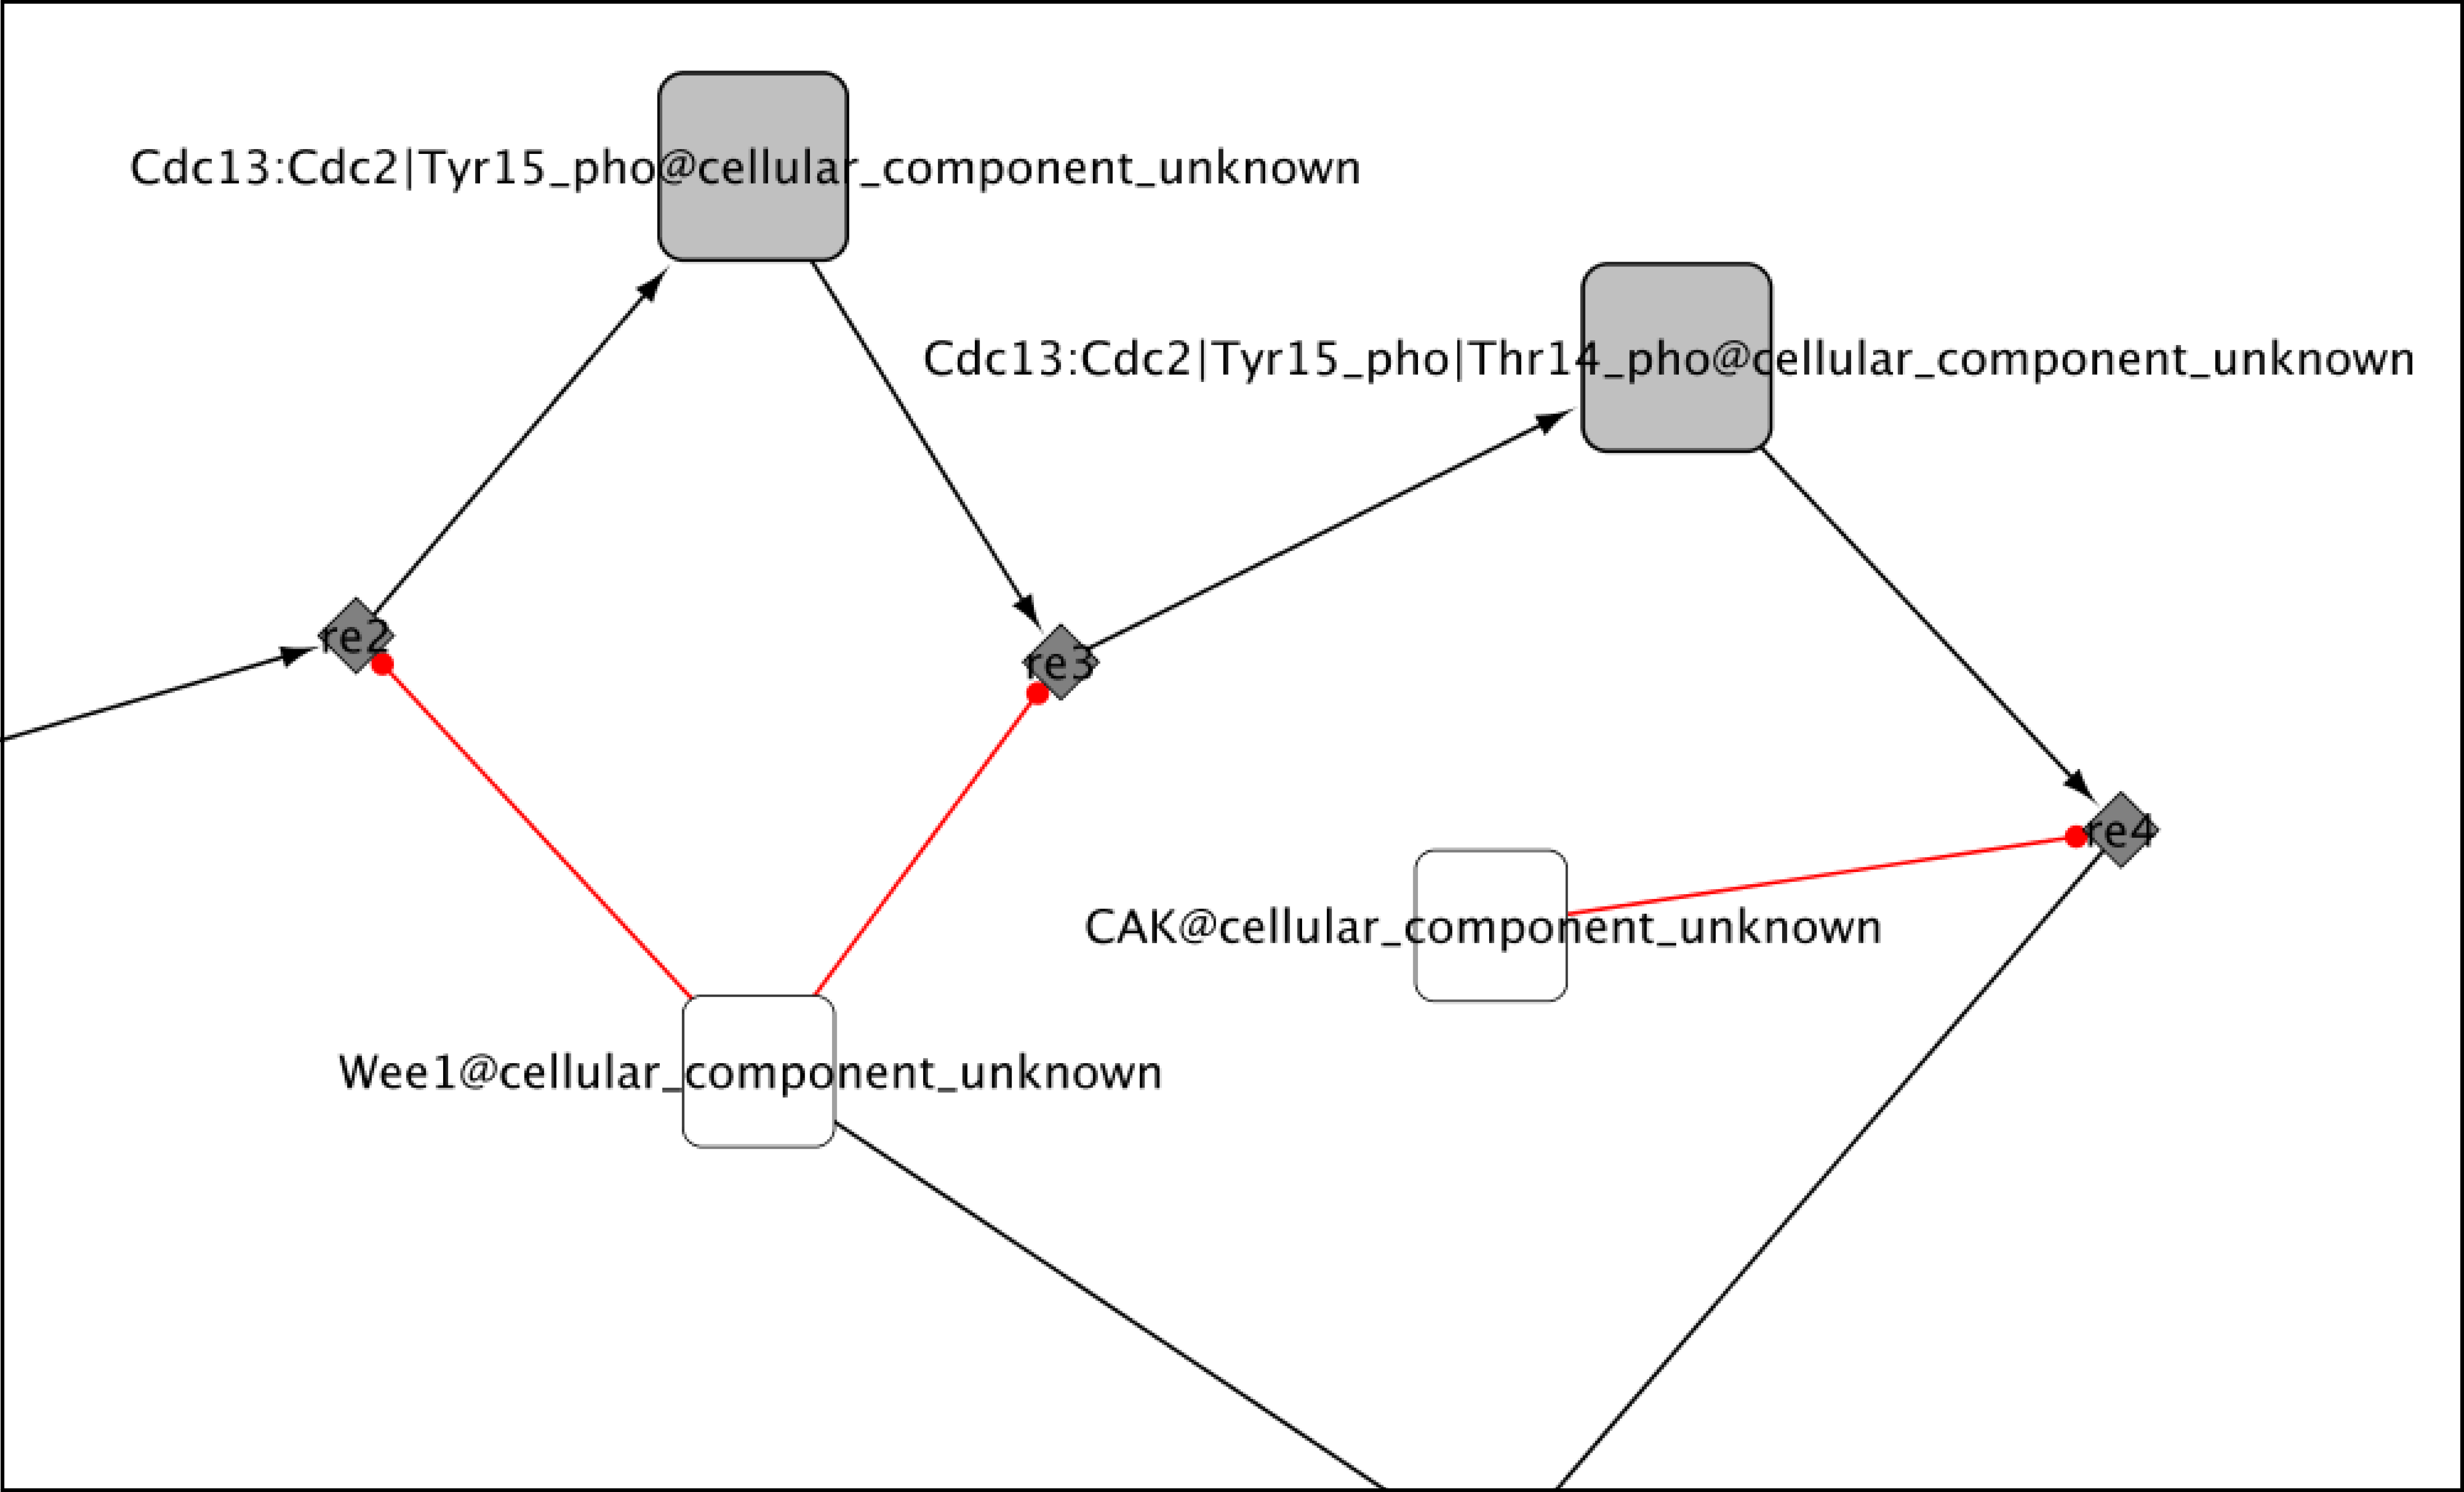
\includegraphics[width=0.7\textwidth]{figures/mphase_biopax.png}}
\end{figure}

\begin{figure}[h]
 \caption{\label{apoptosishierarchical}  \textbf{Apoptosis pathway hierarchical
structure.} Zoom on the BioPAX data extracted from the Reactome database
\cite{joshi2005reactome}. The green nodes represent pathways, the pink
triangular nodes denote steps, while grey nodes indicate reactions.}
 \center{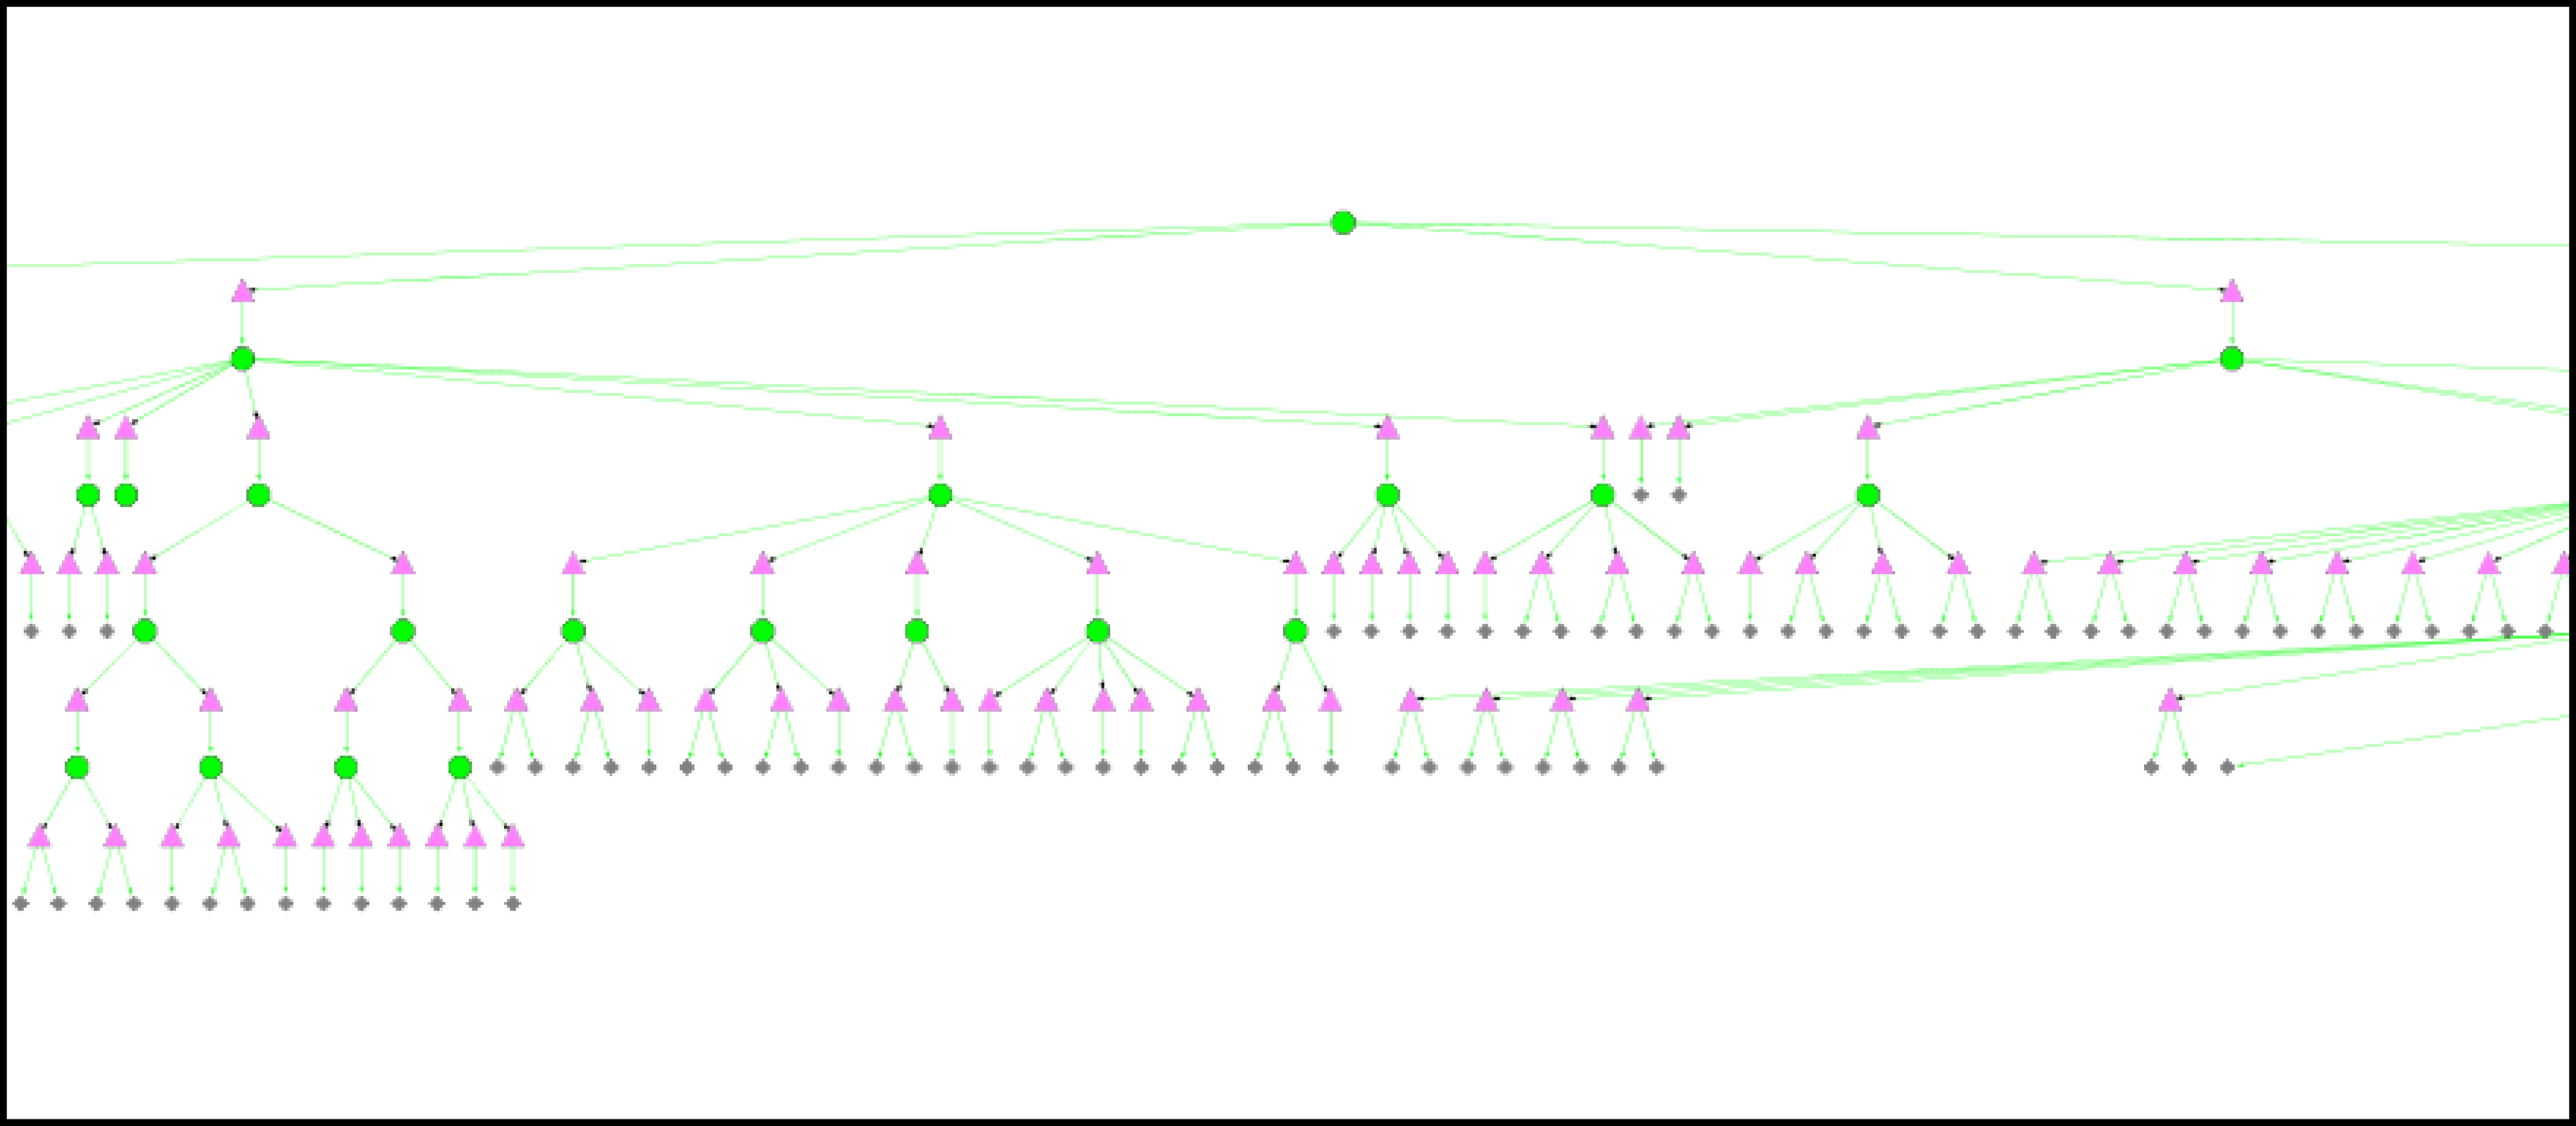
\includegraphics[width=0.7\textwidth]{figures/apoptosis_hierarchical.png}}
\end{figure}


When importing a file, BiNoM is calling a \emph{naming service} function, in
order to create meaningful names for the various entities. More precisely,
entity names are combined with other features such as modifications, compartment
and complexes components. The different features are indicated by special
characters, such as ``@'' for the compartments, ``$|$'' for modifications and
``:'' to delimitate the different members of a protein complex. For example, the
name Cdc25$|$Pho@cytoplasm represent the protein Cdc25 in a phosphorylated
state, located in the cytoplasm, while the name
Cdc13:Cdc2$|$Thr167\_pho@cytoplasm indicate a protein complex located in the
cytosplasm, composed of the protein Cdc13 and the protein Cdc2 phosphorylated at
position 167 on a threonin residue.

BiNoM allows the interconversion of CellDesigner files to BioPAX, and from a BioPAX
reaction network to SBML level 2 (not to the CellDesigner dialect). The
cytoscape networks must be associated to existing CellDesigner or BioPAX files
prior to this operation (see the BiNoM manual for more details). While the
content of BioPAX files can be altered using BiNoM functions, it is not possible
to create a CellDesigner file from scratch or using the graphical notations from
a BioPAX file. In fact there are a couple of typical scenarios where BiNoM I/O
functions can help the user. For example, after the import of a BioPAX file as a
reaction network or a pathway structure, the user can create a subnetwork (or
subpathway) and save it as a new BioPAX file. Another example would be to import
a BioPAX file, select a subnetwork of interest and save it as a SBML file for
the creation of a computational model using an appropriate software package.
At last, a user might want to import a large CellDesigner map and export only a
subnetwork as a new CellDesigner file.  


\subsection*{BiNoM Analysis}
The central goal of the BiNoM software package is to provide efficient methods
and algorithms to reduce the inherent complexity of biological networks into
manageable and meaningful subnetworks. This goal is achieved by a set of
functions included as a built-in structural graph analysis library, taking into
account for some of them the semantics contained in the graph elements. Those
approaches include the analysis of connected and strongly connected components,
pruning the network, decomposition in material components or in cycles, path
analysis and network clustering.

A trivial approach to split a network is to dissociate the unconnected subparts
of the network. A more sophisticated one consist in decomposing the network into
strongly connected components, using the algorithm of Tarjan
\cite{tarjan1972depth}.

It is also possible to prune the network into three different parts:
first all the elements associated with the \emph{input} parts of the network, a
second with all the elements associated with the \emph{output} part and at last
all the elements linked to the central, cyclic part. This type of approach
corresponds to the bow-tie model of Broder and colleagues \cite{broder2000graph}.

The decomposition in material components is using the node name semantics to
isolate subnetworks in which each protein is involved. Major overlaps between
the different subnetworks are to be expected, as some proteins are involved in
several different complexes. The figure~\ref{matcdc2cdc13} is showing two examples of subnetworks
obtained by material components decomposition applied to the cell cycle network
model.
%
% EB: emphasize that BiNoM is not a universal converter.
%

\begin{figure}[h]
 \caption{\label{matcdc2cdc13}  \textbf{Subnetworks obtained after a decomposition in
material components.} The two overlapping subnetworks correspond to the components Cdc13 and
Cdc2.}
 \center{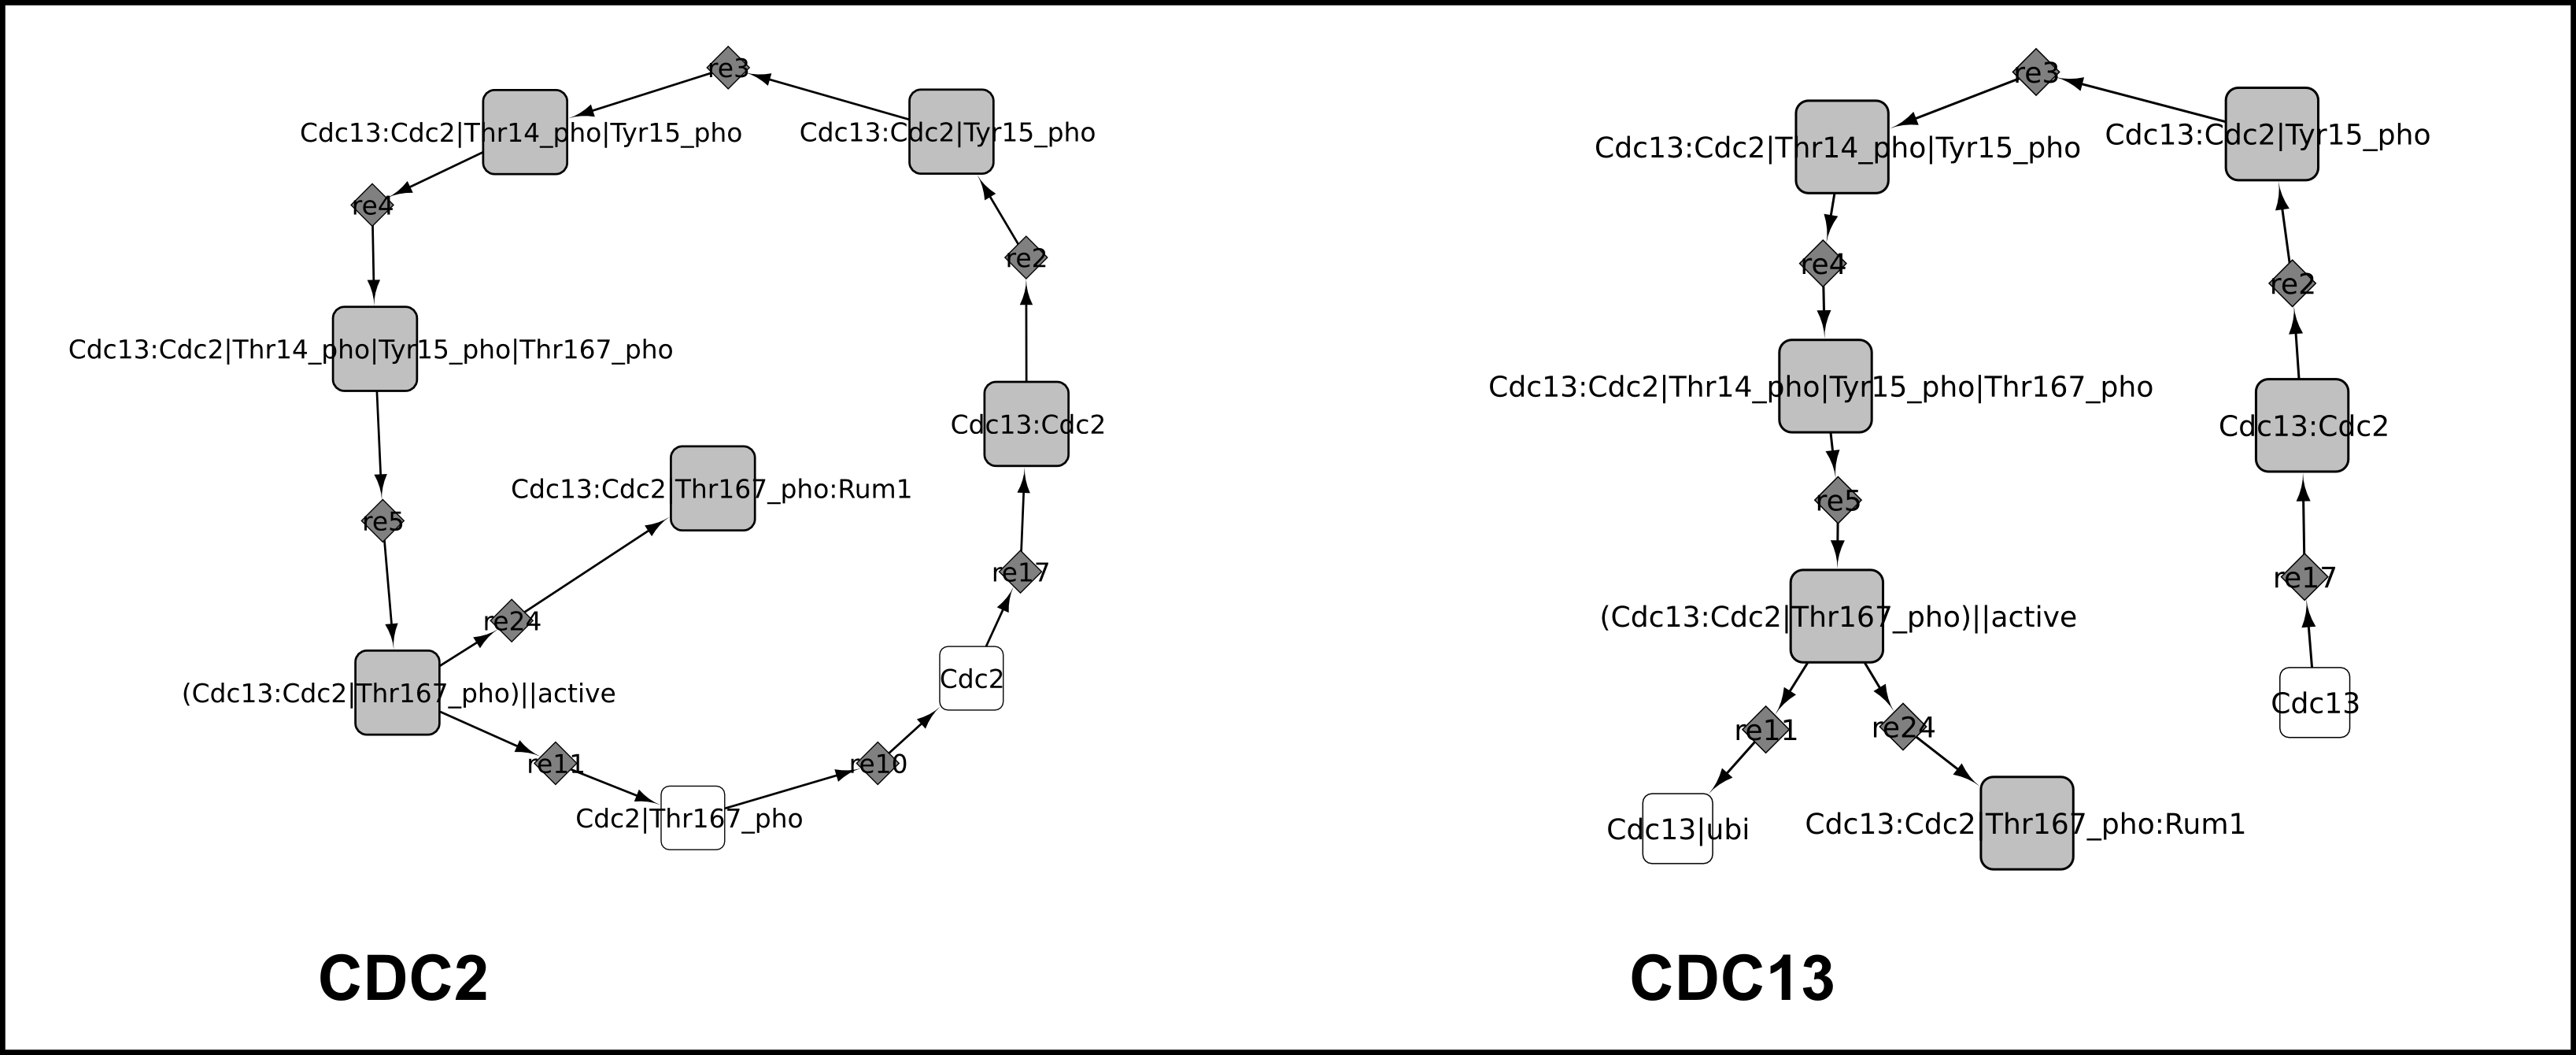
\includegraphics[width=0.7\textwidth]{figures/mat_cdc2_cdc13.png}}
\end{figure}


The cycle decomposition is splitting the network into relevant directed cycles
\cite{gleiss2001relevant}, using a modifed version of the algorithm of Vismara
and colleagues \cite{vismara1997union}. Very often, this approach will represent
the different parts of the life cycle of a given protein or complex. Care must
be taken when applying this approach, as the number of cycles can be huge for
large network structures. For example, it might be preferable to eliminate first
the network hubs, which are by definition highly connected, and also group short
cycles in meta-nodes before applying the procedure. The figure~\ref{mphasecdc25cycles} is showing two
cycles involving CDC25 after a cycle decomposition.

\begin{figure}[h]
 \caption{\label{mphasecdc25cycles}  \textbf{CDC25 subnetworks.}
      Two cycles for the CDC25 protein found after the decomposition of the cell cycle network model of Novak et al. \cite{novak1998model}.}
 \center{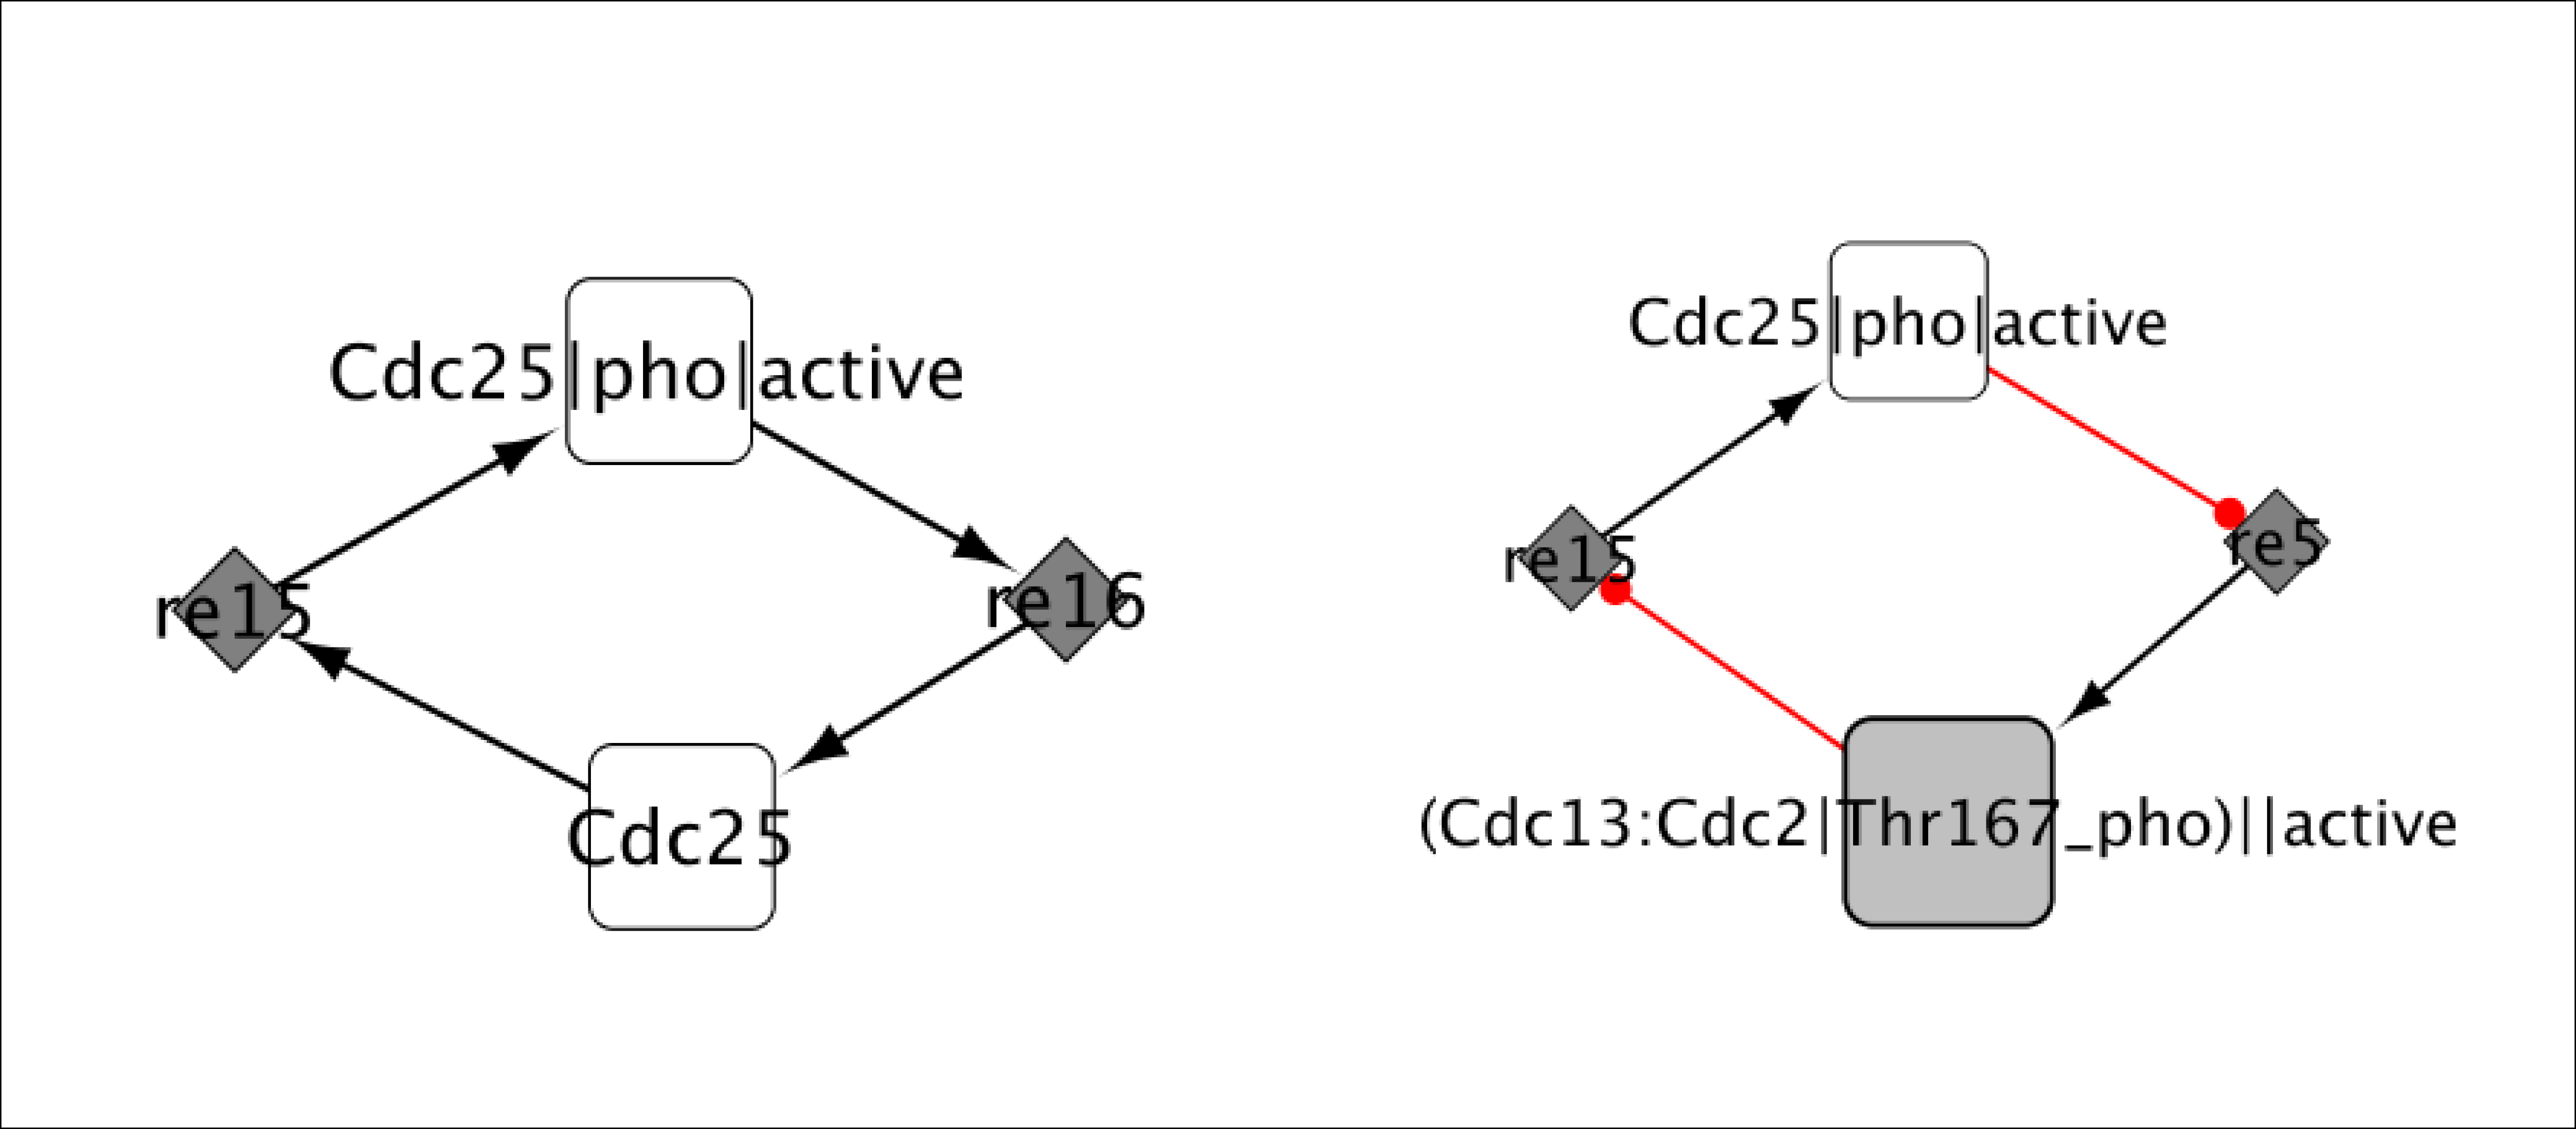
\includegraphics[width=0.7\textwidth]{figures/mphase_cdc25_cycles.png}}
\end{figure}

BiNoM analysis functions also include several classical path analysis
algorithms, such as finding the shortest paths, the suboptimal shortest paths or
all non-intersecting paths [ comment: maybe the priciple of the algorithms
should be explained here in more details]. As usual, some care must be taken
before launching those functions, as the number of paths between nodes can be
very large for big networks.

Obviously, the result of some decomposition functions will result in subnetworks
that share a large number of components, as it is for example often the case
with the decomposition in material components. Therefore, BiNoM also include a
function to \emph{cluster} networks, based on common components such as protein
or protein complexes. To determine the size of the clusters, the user can
specify a percentage of intersection (ranging from 0 to 100\%) that will be used
as a threshold to create the clusters.

%
% this paragraph on PIQuant should be reviewed by GS
%

In this version of BiNoM, we have introduced a novel approach to quantify the
influence of one or more molecular paths on a given set of valuable target
nodes, named PIQuant (Pathway Influence Quantification). A path $k$ is defined
as a the sequence of consecutive connected nodes
between a source node $A$ and a target node $B$ (without repetition of any node
or edge). We also define the activity $\alpha$ of a path as a signed real number
representing for example the expression ratio of a given gene, the sign $\sigma$
of the path as the product of the signs of every edge of the path and finally
the length $\lambda$ of the path as the number of edges in the path. We also
hypothesize that the longer the path is, the lesser the global influence will be
on the target node. Then the PIQuant score for a set of $q$ paths for a given
target node $O$ of interest is defined as:

$$
 PIQuant_{Score} = \sum_{k=1}^{q} \alpha_{k} \sigma_{k} \frac{1}{\lambda_{k}}
$$

For example, a very simple influence network composed of seven nodes is shown on
figure~\ref{piquantnetworks}a. The figures ~\ref{piquantnetworks}b and
~\ref{piquantnetworks}c show 2 paths extracted from this network. Given that the
node AC has an activity value of 2, and that the two paths have the same length
equal to 3, we can calculate the PIQUANT score for the Ph node as:

$$
 PIQuant_{Score} = 2 \cdot 1 \cdot \frac{1}{3} + 2 \cdot (-1) \cdot \frac{1}{3}
= 0.27
$$

In more realistic situations, we will have multiple source nodes with different
activity values, and also multiple target nodes representing phenotypes of
particular nodes of interest. We have implemented in BiNoM a set of functions
that allow users to select source nodes, select target nodes, and choose among
three different options for searching paths (shortest paths, optimal and
suboptimal shortest paths, all non-intersecting paths). The software is then
calculating PIQUANT scores for every target node specified, taking into account
every possible path found by the algorithm. We describe a detailed and concrete
application of the PIQUANT algorithm to a real biological network in the results
section.

\begin{figure}[h]
 \caption{\label{piquantnetworks}  \textbf{A simple influence network.} The 
network is composed of seven nodes and nine edges (a). The two paths (b,c)
extracted from this network start from the source node \textbf{Ac} and end at
the target node \textbf{Ph} (which denotes a phenotype of interest). The node
\textbf{Ac} is the only one for which
an activity value is known (value=2).}
 \center{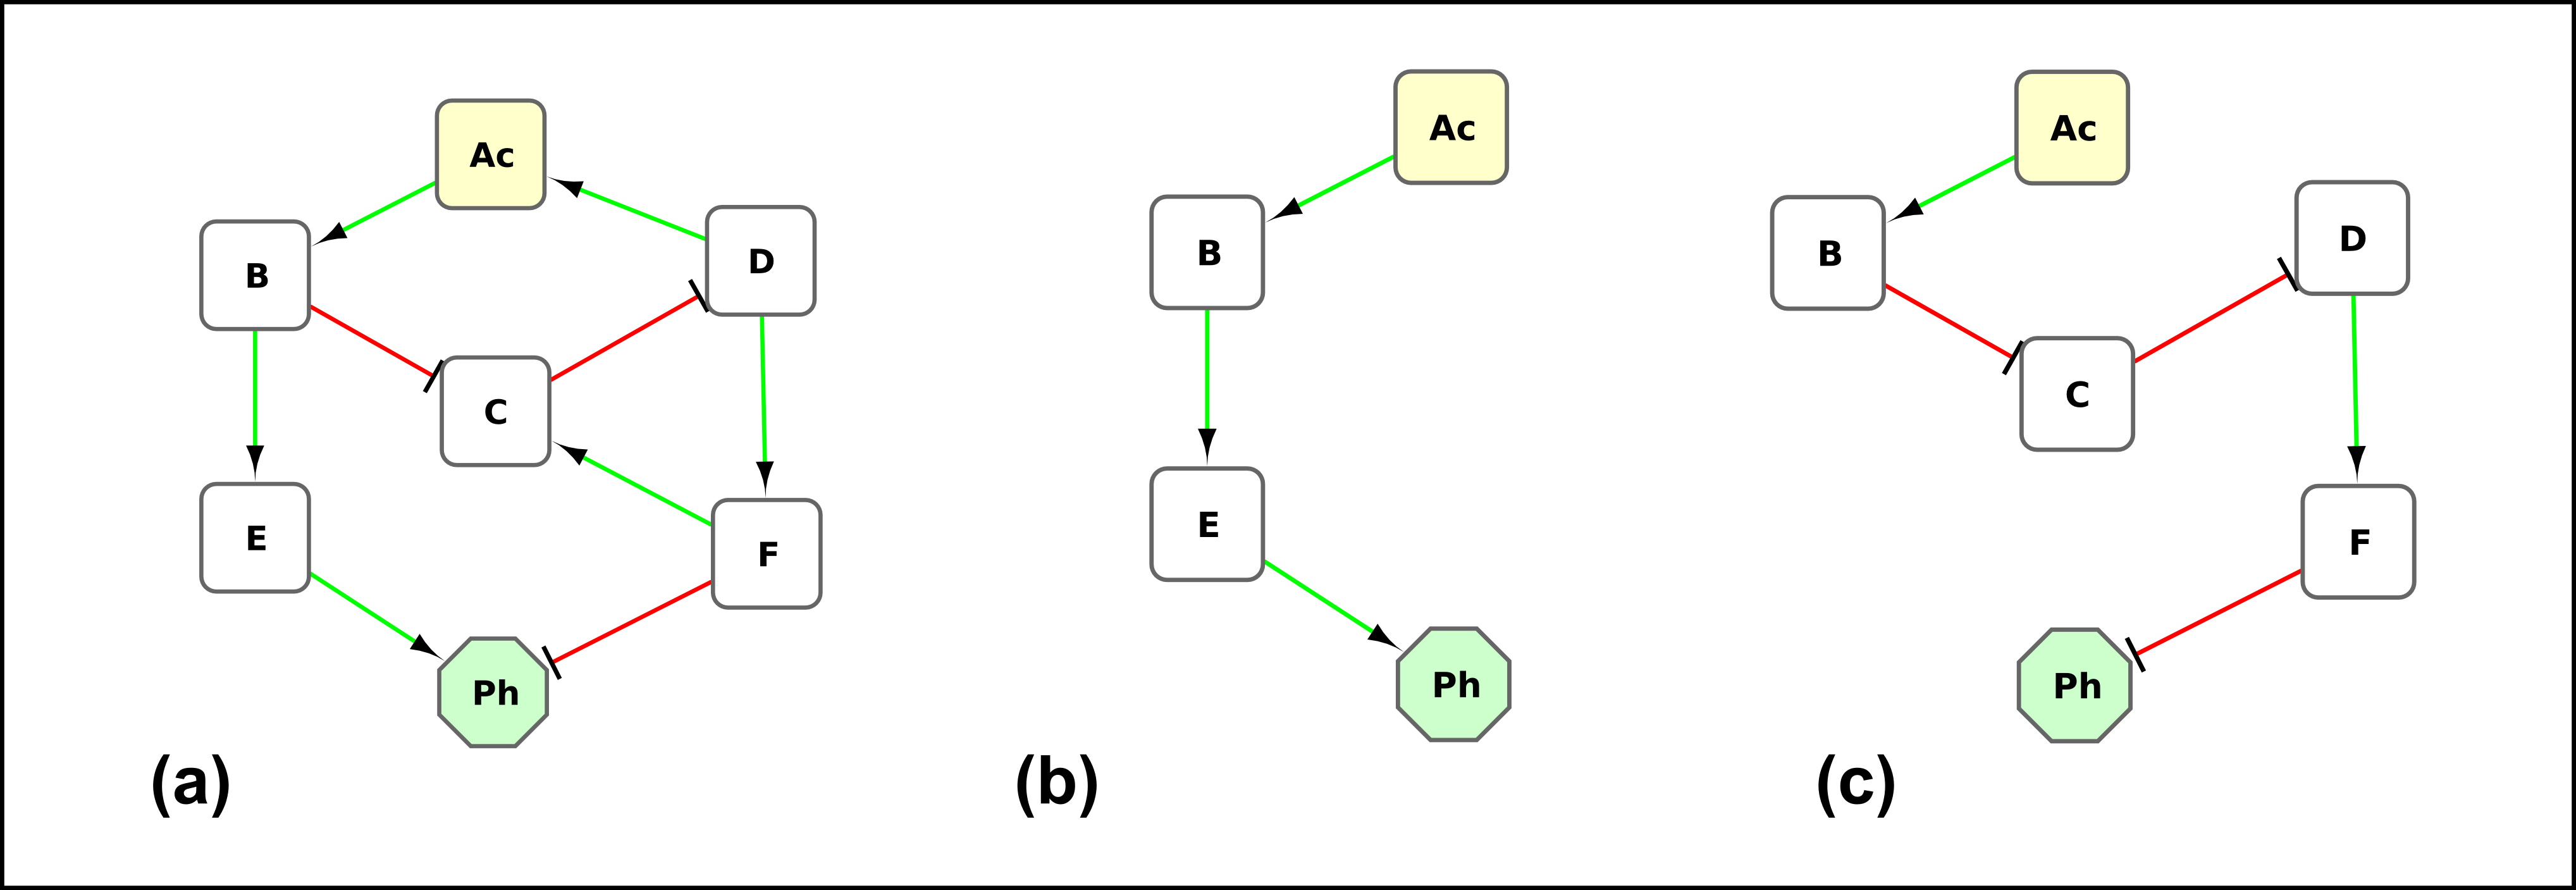
\includegraphics[width=0.7\textwidth]{figures/piquant_networks.png}}
\end{figure}

%
% a short description of the path consistentcy should be added here (GS, EB???)
%

\subsection*{BiNoM BioPAX utils \& query}
The BioPAX format was primarily conceived as a standard facilitating the
exchange of data between various database systems \cite{demir2010biopax}. As a
consequence, this format was designed first to be machine-readable, but was not
intended
to be edited and modified by biologists. Furthermore, due to its adoption by
large biological knowledge repositories, some BioPAX files can be really big,
such as the \textit{Homo sapiens} network from the reactome database
\cite{joshi2005reactome} that has more than 6,000 reactions involving more than
8,000 different species (proteins, RNA molecules, metabolites, etc.).

BiNoM implements a set of functions precisely aiming to allow end users to
easily visualize and modify BioPAX files. To the best of our knowledge, there is
no other software package allowing to view, query and edit BioPAX files than
BiNoM at the moment.The functions are using
java classes introspection techniques to build a BioPAX class tree. Then, the
content of the file can easily be accessed. For example, the figure~\ref{biopaxtrailprop} is
showing all the informations linked to the TRAIL protein, after a call to the
BioPAX property
editor function of the BiNoM menu. Details are given in the BiNoM manual on how
to to display valid attributes and edit them, and also how to visualize the
complete BioPAX tree.


\begin{figure}[h]
 \caption{\label{biopaxtrailprop}  \textbf{Extra Information linked to the TRAIL protein.}
      The informations are automatically extracted from the BioPAX file upon
import with the BiNoM I/O functions.}
 \center{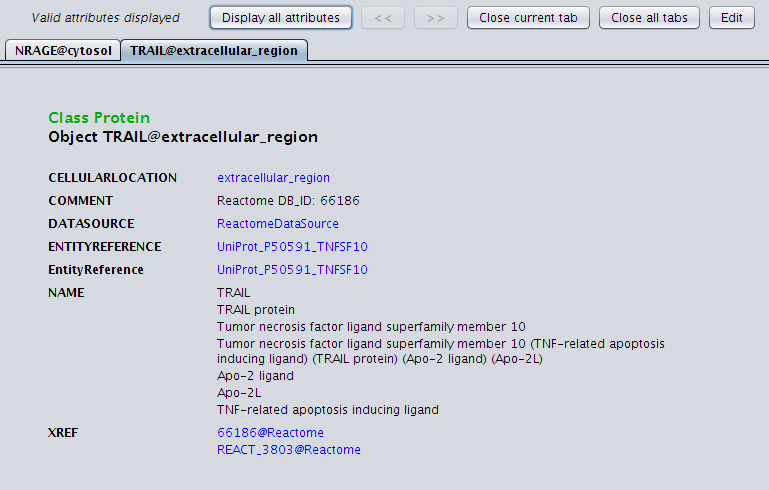
\includegraphics[width=0.7\textwidth]{figures/biopax_trail_prop.png}}
\end{figure}


The BioPAX Query functions in BiNoM allow the user to work with potentially huge
BioPAX data files and extract the relevant information, by querying an index and
retrieving data from it. The index corresponds to a mapping of the content of
the BioPAX file on a labeled graph (an index file is created and saved, using
the XGMML format). Various statistics can be displayed on the content of the
index, such as the number of proteins, complexes, reactions, publications, etc.
To start extracting relevant informations, the user can query the index by gene
name (and/or by any synonym of the gene) and start building a network centered
around this molecule of interest. The extension of the network is done by adding
different type of entities: complexes where the molecule of interest is
involved, chemical species, reactions (with the possibility of including all the
sources and targets of the reactions) and related publications. The figure~\ref{smaccomplexes}
is showing an example of a small network extracted from the human apoptosis
pathway downloaded from the Reactome database \cite{joshi2005reactome}, and
centered on the SMAC protein, with all the protein complexes where
this protein is involved that were added using the BiNoM functions.


\begin{figure}[h]
 \caption{\label{smaccomplexes}  \textbf{SMAC pathway subnetwork.}
      Subnetwork extracted from the human Apoptosis pathway, starting with the
SMAC protein and expanding to all protein complexes where this
molecule is involved using the BiNoM Query functions.}
 \center{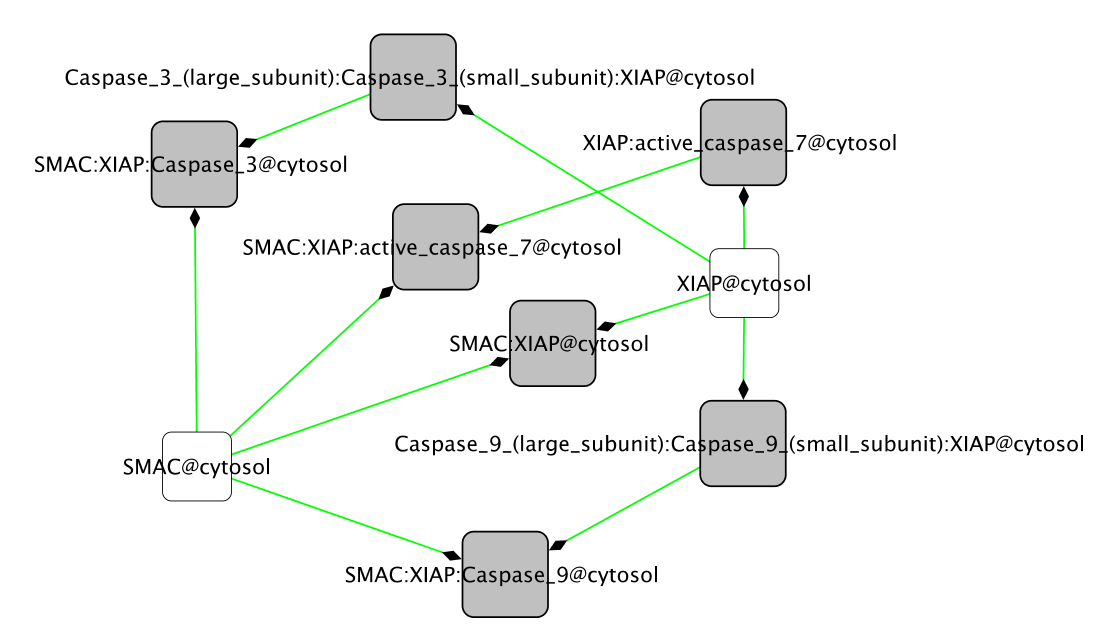
\includegraphics[width=0.7\textwidth]{figures/smac_complexes.png}}
\end{figure}


\subsection*{BiNoM Module manager}
The application of selected BiNoM analysis algorithms to a large network map,
usually followed by manual curation, results in the creation of a certain number
of connected network \emph{modules}. Most of the modules represent a detailed
sequence of events that occur with a particular protein or protein complex,
whose name can then be used to represent the whole module. This way, a
simplified representation of a complex map can be produced, using the modules
and their relationships as an abtracted version of the comprehensive network
\cite{calzone2008comprehensive}.

To facilitate the creation and management of modules, we have used in this
version of BiNoM a new feature introduced in recent versions of Cytoscape (as of
version 2.7) \cite{cline2007integration}, known as \emph{nested} networks. This
feature allows to embed any cytoscape network in a (meta)node. It was
introduced to allow the creation of network hierarchies and circular
relationships. In BiNoM, we use this feature to facilitate the process of
modularization of a large network. The BiNoM module manager integrates a set of
funtions that allow to easily create a network from a list of subnetworks,
packing individual nodes, merging different subnetworks, displaying informations
about metanodes and calculating intersection between subnetworks.

\subsection*{BiNoM Utilities}
This set of functions correspond to various small utilities that are not
implemented yet in Cytoscape, but might be very useful for the analysis and
manipulation of networks. For example, it is possible to automatically select
the edges between two nodes, generate the network corresponding to the double
network differences between two networks A and B, or update all the networks of
a session after some changes have been made. The BiNoM utilities also implements
clipboard related functions, giving the possibility to copy, add and paste
selected nodes and edges and also to show the clipboard content. 


\section*{Results and Discussion}

%
% LC: give an extended description of the biological context.
%
% expliquer le cycle cellulaire et le role de RB dans le cycle (LC)
% 

We propose to study a reaction network of the regulation of the protein RB (also
referred to as RB1) \cite{calzone2008comprehensive} as an example of the use of
BiNoM functions. The complete network contains about 78 proteins, 208 chemical
species, and 165 biochemical reactions. For this study, we choose to concentrate
on the G1 to S transition. For that, we used the intersection of the 208 species
of RB/E2F network and the 280 species listed in Reactome for the G1-S transition
(referred to as \emph{Mitotic G1 G1/S phases} in Reactome). The resulting
subnetwork contains 38 proteins, 98 chemical species, and 100 biochemical
reactions (Figure~\ref{g1s}).

%
% include new code to convert bioch to influence network (AZ)
% compare result with biocham conversion (LC, AZ)
% describe how the network is build (LC)
%

\begin{figure}[h]
 \caption{\label{g1s}  \textbf{G1/S network.}
	Network of the G1 to S transition corresponding to the intersection of
RB-E2F network and G1/S network extracted from Reactome.}
 \center{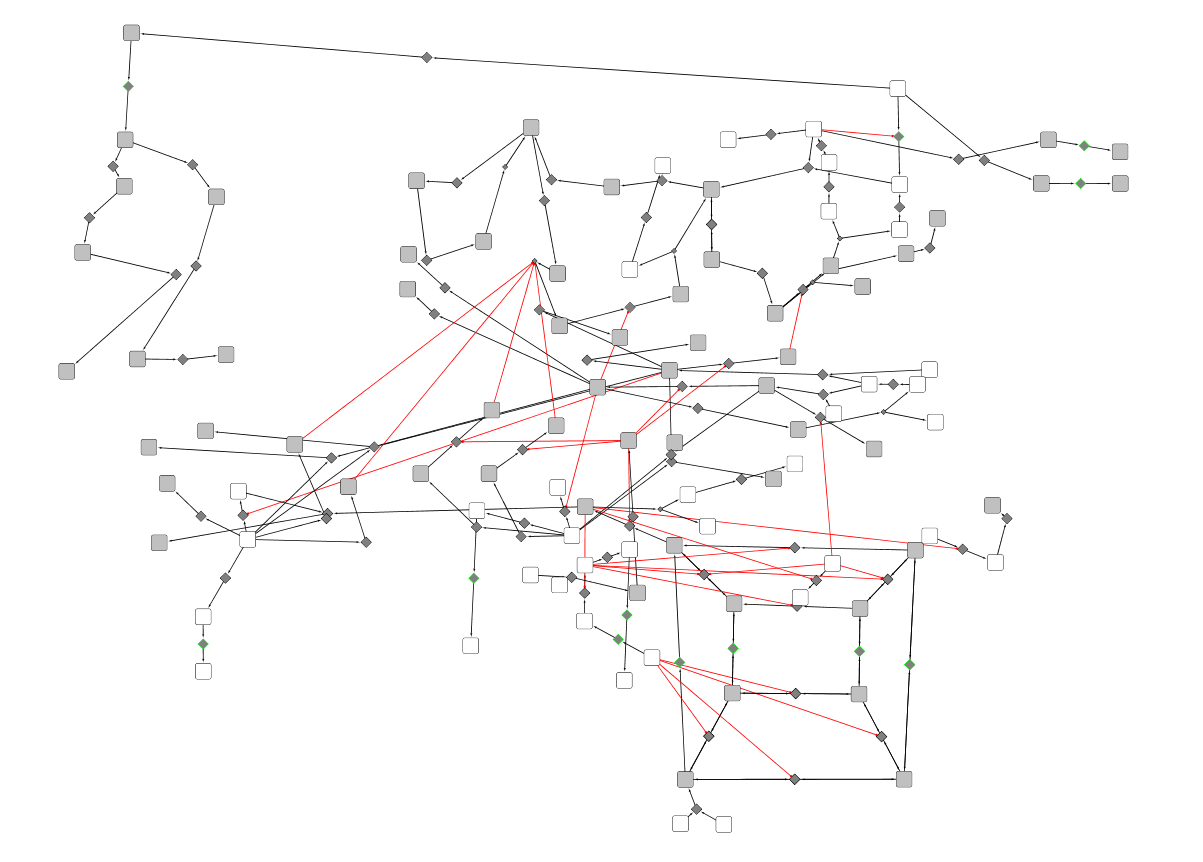
\includegraphics[width=0.7\textwidth]{figures/G1S.png}}
\end{figure}


\subsection*{Application of PIQuant on 2 GS networks (comprehensive + modular
network), data from Stransky.}
%
% PIQuant analysis here (GS)
%

\subsection*{Modularization} 

The raw G1/S network is very detailed and may be hard to read at a first glance.
To facilitate the analysis of the content, we propose to organise the reaction
network as a modular network. The species are clustered in groups, referred to
as modules, in an semi-automatic manner, using BiNoM functions and biological knowledge. Each module represent in fact a
sequence of events occuring with a particular protein. The modules are then
linked by activating or inhibiting influences according to the informations
contained in the original diagram or derived from previous biological knowledge.

Briefly, we first decomposed the global network into its different components,
by using name semantics to isolate the sub-networks in which
each protein is involved. The 36 networks that are created this way may share a
lot of common species, so we went further
by clustering the subnetworks having at least 25\% of common species. We renamed
the 7 clusters obtained with a name that illustrate the content and the main
function of the clusters (such as E2F1\_RB, Wee1, etc.). Then, we checked the
content of each module, making modifications if necessary. For example, the
module E2F1\_RB is
further decomposed in three different modules containing the proteins RB, E2F1
and E2F6. Finally, we created a final modular view, where we integrate the
subnetworks we have previously created using a set of BiNoM functions for the
management of modules. Our final modular view is composed of 9 modules, with 22
edges connecting them (Figure~\ref{g1smodular}). A detailed tutorial on the construction of
this modular network using BiNoM is described in the supplementary methods.


\begin{figure}[h]
 \caption{\label{g1smodular}  \textbf{Modular view of the G1/S network.}
	Modular representation of the G1/S network, created by using a set of
different BiNoM functions. Each node (pictured as a green octagon), represents a
different module, or subnetwork. The edges connecting the modules represent the
 known influences between modules. }
 \center{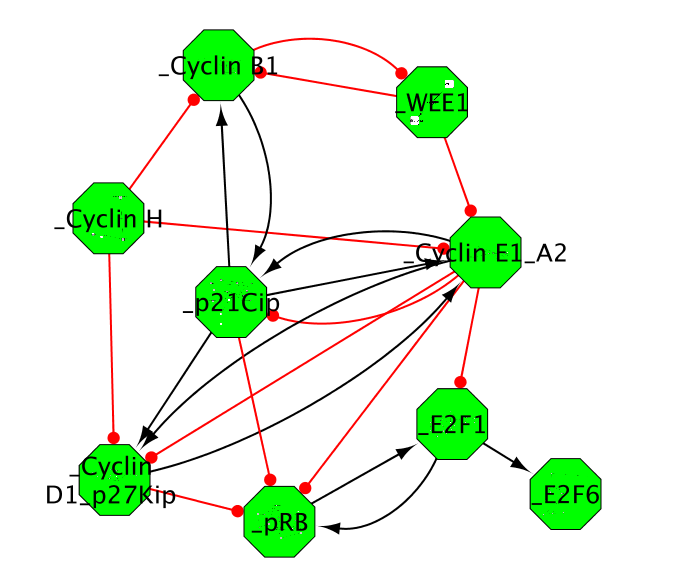
\includegraphics[width=0.7\textwidth]{figures/G1S_modular.png}}
\end{figure}


\section*{Conclusions}

bla bla bla

\section*{Availability and requirements}

\begin{itemize}
\item Project name: BiNoM
\item Project home page: \url{http://bioinfo-out.curie.fr/projects/binom/}
\item Operating system(s): Platform independent
\item Programming language: java
\item Other requirements: java 1.5 or higher, Cytoscape 2.7 or higher
\item License: GNU LGPL
\item Any restriction to use by non-academics: none
\end{itemize}




% \section*{Section title}
% \subsection*{Sub-heading for section}
% \subsubsection*{Sub-sub heading for section}
% \subsubsection*{Sub-sub-sub heading for section}

\bigskip

%%%%%%%%%%%%%%%%%%%%%%%%%%%%%%%%
\section*{Author's contributions}
    Text for this section \ldots

    

%%%%%%%%%%%%%%%%%%%%%%%%%%%
\section*{Acknowledgements}
  \ifthenelse{\boolean{publ}}{\small}{}
  EB, LC, DR and AZ are members of the team ‘‘Computational Systems Biology of
Cancer,’’ Equipe labellisée par la Ligue Nationale Contre le Cancer.
 
%%%%%%%%%%%%%%%%%%%%%%%%%%%%%%%%%%%%%%%%%%%%%%%%%%%%%%%%%%%%%
%%                  The Bibliography                       %%
%%                                                         %%              
%%  Bmc_article.bst  will be used to                       %%
%%  create a .BBL file for submission, which includes      %%
%%  XML structured for BMC.                                %%
%%  After submission of the .TEX file,                     %%
%%  you will be prompted to submit your .BBL file.         %%
%%                                                         %%
%%                                                         %%
%%  Note that the displayed Bibliography will not          %% 
%%  necessarily be rendered by Latex exactly as specified  %%
%%  in the online Instructions for Authors.                %% 
%%                                                         %%
%%%%%%%%%%%%%%%%%%%%%%%%%%%%%%%%%%%%%%%%%%%%%%%%%%%%%%%%%%%%%

\newpage
{\ifthenelse{\boolean{publ}}{\footnotesize}{\small}
 \bibliographystyle{bmc_article}  % Style BST file
  \bibliography{binom2} }     % Bibliography file (usually '*.bib' ) 

%%%%%%%%%%%

\ifthenelse{\boolean{publ}}{\end{multicols}}{}

%%%%%%%%%%%%%%%%%%%%%%%%%%%%%%%%%%%
%%                               %%
%% Figures                       %%
%%                               %%
%% NB: this is for captions and  %%
%% Titles. All graphics must be  %%
%% submitted separately and NOT  %%
%% included in the Tex document  %%
%%                               %%
%%%%%%%%%%%%%%%%%%%%%%%%%%%%%%%%%%%

%%
%% Do not use \listoffigures as most will included as separate files

%\section*{Figures}
%  \subsection*{Figure x - title}
%      Description.


%%%%%%%%%%%%%%%%%%%%%%%%%%%%%%%%%%%
%%                               %%
%% Tables                        %%
%%                               %%
%%%%%%%%%%%%%%%%%%%%%%%%%%%%%%%%%%%

%% Use of \listoftables is discouraged.
%%
%\section*{Tables}
%  \subsection*{Table 1 - Sample table title}
%    Here is an example of a \emph{small} table in \LaTeX\ using  
%    \verb|\tabular{...}|. This is where the description of the table 
%    should go. \par \mbox{}
%    \par
%    \mbox{
%      \begin{tabular}{|c|c|c|}
%        \hline \multicolumn{3}{|c|}{My Table}\\ \hline
%        A1 & B2  & C3 \\ \hline
%        A2 & ... & .. \\ \hline
%        A3 & ..  & .  \\ \hline
%      \end{tabular}
%      }



%%%%%%%%%%%%%%%%%%%%%%%%%%%%%%%%%%%
%%                               %%
%% Additional Files              %%
%%                               %%
%%%%%%%%%%%%%%%%%%%%%%%%%%%%%%%%%%%

\section*{Additional Files}
  \subsection*{Supplementary methods}
	Detailed tutorial for the creation of a modular view of the G1/S network using BiNoM functions.

\end{bmcformat}
\end{document}







